\chapter{List of Resources}

This chapter provides a detailed overview of the hardware, software, and supporting materials required for the development of the proposed foot-wearable biomedical monitoring system. The resources listed below encompass all necessary components for data acquisition, signal processing, communication, analysis, and application development. Each item includes a brief description, approximate cost (if known), and whether it represents a new learning requirement for the team.

\newpage
\section{Hardware Components}

Table~\ref{tab:hardware} lists the hardware components used in the prototype of the device. These components include sensors, electronic modules, power systems, and mechanical materials that were integrated into the wearable.

\begingroup
\footnotesize
\setlength{\tabcolsep}{3.5pt}%
\setlength{\LTpre}{6pt}%
\setlength{\LTpost}{6pt}%
\setlength{\LTleft}{0pt}%
\setlength{\LTright}{0pt}%
\renewcommand{\arraystretch}{1.2}%
\begin{longtable}{|>{\raggedright\arraybackslash}p{2.85cm}|>{\raggedright\arraybackslash}p{8.55cm}|>{\raggedright\arraybackslash}p{1.95cm}|>{\centering\arraybackslash}p{1.25cm}|}
\caption{Hardware Components and Materials.}\label{tab:hardware}\\
\hline
\textbf{Component} & \textbf{Description / Purpose} & \textbf{Approx.\ Price (USD)} & \textbf{New Tool?} \\
\hline
\endfirsthead
\multicolumn{4}{c}%
{{\tablename\ \thetable{} --- \textit{continued from previous page}}} \\
\hline
\textbf{Component} & \textbf{Description / Purpose} & \textbf{Approx.\ Price (USD)} & \textbf{New Tool?} \\
\hline
\endhead
\hline
\multicolumn{4}{r}{\small\emph{Continued on next page\ldots}} \\
\endfoot
\hline
\endlastfoot
Arduino Nano 33 BLE & Main microcontroller with integrated BLE, motion sensors, and sufficient processing for biomedical data handling. & 35 & Yes \\ \hline
Force Sensitive Resistors (Velostat) & Placed under the foot to measure static plantar pressure distribution used for ataxia diagnosis through AI. & 5--10 each & Yes \\ \hline
Textile-Flexible Stretch Sensors & Detect ankle circumference variation to quantify edema severity and fluid retention. & 8--12 & Yes \\ \hline
PPG Sensor (MAX30102) & Captures PPG signals to measure SpO$_2$, heart rate, and estimate BP via AI models. & 10--20 & Yes \\ \hline
Rechargeable Li-Po Battery (3.7 V, 1200--2000 mAh) & Supplies power to the wearable during continuous operation. & 10--20 & No \\ \hline
Charging Module TP4056 and Step-up Converter & Ensures safe charging and voltage regulation of the power system. & 5 & No \\ \hline
Elastic Textile (Cotton, Lycra, Conductive Fabric) & Forms the wearable layer embedding sensors for comfort and flexibility. & 10--15 & Yes \\ \hline
Multimeter and Soldering Tools & Required for circuit testing, wiring, and assembly of the prototype. & -- & No \\ \hline
Samsung Smartphones (Pre-owned) & Used for continuous real-time testing of the Android application throughout development and integration phases. & 0 & No \\ \hline
Reference Shoe & A standard commercial shoe used to establish the mechanical baseline and spatial reference for sensor placement and plantar pressure calibration. & 33 & No \\ \hline
3D-Printed Foot Prototype & An anatomically shaped foot model fabricated via 3D printing, used for reproducible sensor calibration and plantar pressure testing. & -- & Yes \\ \hline
Analog Multiplexers (e.g.\ 16-channel CD74HC4067-class ICs) & Used to scan the Velostat plantar-pressure matrix by addressing rows and multiplexing column readout to a single ADC input, reducing pin count on the microcontroller. & 4--10 & Yes \\ \hline
Inertial Measurement Unit (Bosch BMI270) & Built into the Arduino Nano 33 BLE board; provides accelerometer and gyroscope data for steps, motion, and gait-related streams via the \texttt{Arduino\_BMI270\_BMM150} library. & -- (included with board) & Yes \\ \hline
\textbf{Estimated Total} & & \textbf{$\approx$ 200--250} & \\
\hline
\end{longtable}
\endgroup
\vspace{2pt}

\section{Software Tools}

Table~\ref{tab:software} outlines the software and analytical tools used throughout the project for firmware development, signal analysis, dashboard design, machine learning model training, and mobile application development.

\begingroup
\footnotesize
\setlength{\tabcolsep}{3.5pt}%
\setlength{\LTpre}{6pt}%
\setlength{\LTpost}{6pt}%
\setlength{\LTleft}{0pt}%
\setlength{\LTright}{0pt}%
\renewcommand{\arraystretch}{1.2}%
\begin{longtable}{|>{\raggedright\arraybackslash}p{2.85cm}|>{\raggedright\arraybackslash}p{8.55cm}|>{\raggedright\arraybackslash}p{1.95cm}|>{\centering\arraybackslash}p{1.25cm}|}
\caption{List of Software and Analytical Tools.}\label{tab:software}\\
\hline
\textbf{Software Tool} & \textbf{Purpose / Application} & \textbf{License / Cost} & \textbf{New Tool?} \\
\hline
\endfirsthead
\multicolumn{4}{c}%
{{\tablename\ \thetable{} --- \textit{continued from previous page}}} \\
\hline
\textbf{Software Tool} & \textbf{Purpose / Application} & \textbf{License / Cost} & \textbf{New Tool?} \\
\hline
\endhead
\hline
\multicolumn{4}{r}{\small\emph{Continued on next page\ldots}} \\
\endfoot
\hline
\endlastfoot
Arduino IDE & Used for firmware programming, sensor data acquisition, and BLE communication. & Free & No \\ \hline
MATLAB / LabVIEW & Used for modeling, simulation, and preprocessing of biomedical signals. & Academic License & Yes \\ \hline
Python (NumPy, Pandas, SciPy, Scikit-learn, PyTorch) & Enables AI model training for ataxia detection, edema quantification, and blood pressure estimation. & Free & Yes \\ \hline
Google Colab (Pro) & Cloud-based GPU environment used for training and evaluating machine learning models. & \$11/month $\times$ 4 months & Yes \\ \hline
Android Studio & Integrated development environment used for building and testing the SoleMate Android application. & Free & Yes \\ \hline
GitHub Copilot & AI-assisted coding tool used to accelerate debugging and assist with unfamiliar Android APIs and syntax. & Free & Yes \\ \hline
Railway & Cloud platform used to securely host environment variables and backend service keys required for email generation. & Free & Yes \\ \hline
SendGrid & Email delivery service integrated into the alert system to send automated notifications when alerts are triggered. & Free & Yes \\ \hline
Visily & UI/UX prototyping tool used to create wireframes and screen flows for the application before implementation in Android Studio. & Free & Yes \\ \hline
Fusion 360 & CAD software used to design the 3D model of the anatomical foot prototype prior to fabrication. & Academic License & Yes \\ \hline
Custom Dashboard & Cloud-based platform for real-time data monitoring and alert visualization. & Free & Yes \\ \hline
Excel / Google Sheets & Used for data logging, analysis, and maintaining the Bill of Quantities. & Free & No \\ \hline
GitHub / Git & Used for collaborative code management, version control, and documentation. & Free & No \\ \hline
Overleaf (LaTeX) & For technical report and documentation preparation. & Free & No \\ \hline
Kotlin and Gradle (Android) & Primary application language and build system used with Android Studio for the SoleMate mobile app. & Free & Yes \\ \hline
Google Play services (Auth) & \texttt{com.google.android.gms:play-services-auth} dependency used for Google account sign-in flows integrated with the application. & Free (Google Play policy / developer console as applicable) & Yes \\ \hline
Arduino firmware libraries (ArduinoBLE, Wire, IMU, crypto) & Third-party and bundled libraries used in embedded firmware: \texttt{ArduinoBLE} for Bluetooth Low Energy, \texttt{Wire} for I\textsuperscript{2}C, \texttt{Arduino\_BMI270\_BMM150} for the onboard IMU, and the Arduino Cryptography library stack for AES-128-CBC and related primitives used with secure BLE payloads. & Free & Yes \\ \hline
Cuirkit & Web-based tool used to draw and document circuit schematics (plantar matrix, flex interfaces, charging/power) as referenced in the design-tools section of this chapter. & Free & Yes \\ \hline
\textbf{Estimated Total} & & \textbf{$\approx$ \$44} & \\
\hline
\end{longtable}
\endgroup

\section{Supporting Equipment and Materials}

In addition to the main hardware and software, several auxiliary resources are required during the design and testing phases:
\begin{itemize}[leftmargin=1.5cm]
    \item \textbf{Prototyping materials:} jump wires, resistors, connectors, headers.
    \item \textbf{Protective coating:} silicone film or textile lamination for moisture resistance.
    \item \textbf{Foot dummy / anatomical model:} fabricated via 3D printing using a Fusion 360 design, used for calibration of plantar and circumference sensors under repeatable conditions.
    \item \textbf{Testing tools:} oscilloscopes, logic analyzers, or other lab instruments (if available).
\end{itemize}



\begin{comment}
\section{Design Tools}

\subsection{Interface and Dashboard Design Tools}

\noindent During the early phase of the mobile application design, Visily was used to build the main user interface (UI) and dashboard structure. It supported quick prototyping, which helped in creating the initial screen flow and overall visual idea of the app. The design aimed to make the application simple and easy to use, with key features like real-time monitoring, data display, and system status placed where users could access them easily. \\

\noindent Visily's drag-and-drop features made it convenient to try out different layouts, visual components, and screen arrangements, giving a clear picture of how the app would appear and operate during the beginning stages. After completing the first design, it became the base for continued development in Android Studio. \\

\noindent As the project moved forward, the design was improved and adjusted to match its specific requirements. Input from testing, functional needs, and performance factors resulted in several UI updates, such as changes to the navigation flow, button structure, and screen interactions. These revisions helped ensure that the final application satisfied both the technical requirements and the intended user experience. \\

\subsection{Cuirkit for Circuit Schematic Design}

\noindent Cuirkit was used to prepare the circuit schematics and connection diagrams of the main hardware subsystems developed for SoleMate. It provided a clear visual representation of the electrical layout of the prototype, which helped the team organize sensor connections, verify pin assignments, and document the integration of the different modules used throughout the system. The generated schematics were particularly useful during debugging and testing, since they offered a structured reference for wiring, power routing, and subsystem interfacing.

\noindent One of the main schematics created using Cuirkit was the Velostat-based plantar-pressure sensing circuit shown in Fig.~\ref{fig:velostat_schematic}. This schematic illustrates the pressure acquisition setup used to reconstruct plantar-pressure frames from the sensing matrix. The design includes the Velostat sensing layer, the associated conductive traces, and the multiplexing arrangement used to scan the matrix while reducing the number of required microcontroller pins. By organizing the matrix rows and columns through multiplexers, the circuit enables sequential sampling of the pressure nodes and supports the generation of plantar-pressure heatmaps for gait analysis.

\begin{figure}[H]
    \centering
    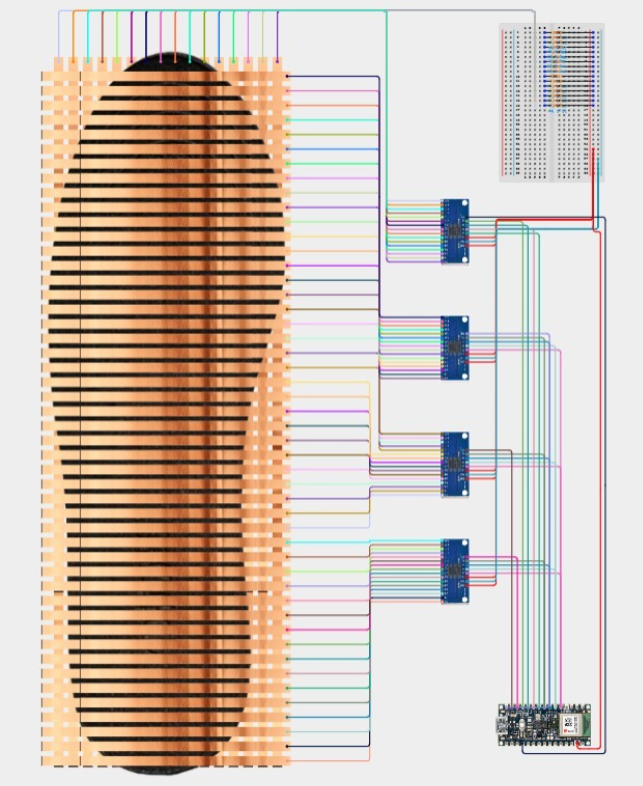
\includegraphics[width=0.82\textwidth]{FYP_Template_Spring/Figures/velostat circuit.png}
    \caption{Cuirkit schematic of the Velostat-based plantar-pressure sensing circuit used for pressure acquisition and heatmap generation.}
    \label{fig:velostat_schematic}
\end{figure}

\noindent TO BE CHANGED!! FIGURES ARE TO BE CHANGED BASED ON OUR LAST CONFIG + THE EXPLANATION SHOULD BE MORE DETAILED IF U WANT GUYS BS LA NE3TEMED AAL FINAL DESIGN OF EACH CIRCUIT

\noindent Another schematic prepared using Cuirkit was the flex-sensor interface circuit shown in Fig.~\ref{fig:flex_schematic}. This diagram documents the connection of the flex sensors used for swelling detection. The circuit was designed so that changes in flex-sensor resistance could be translated into voltage variations readable by the microcontroller through analog input pins. This schematic helped clarify the resistor connections, signal paths, and sensor interfacing required for the swelling-detection subsystem, making the implementation and testing process more organized.

\begin{figure}[H]
    \centering
    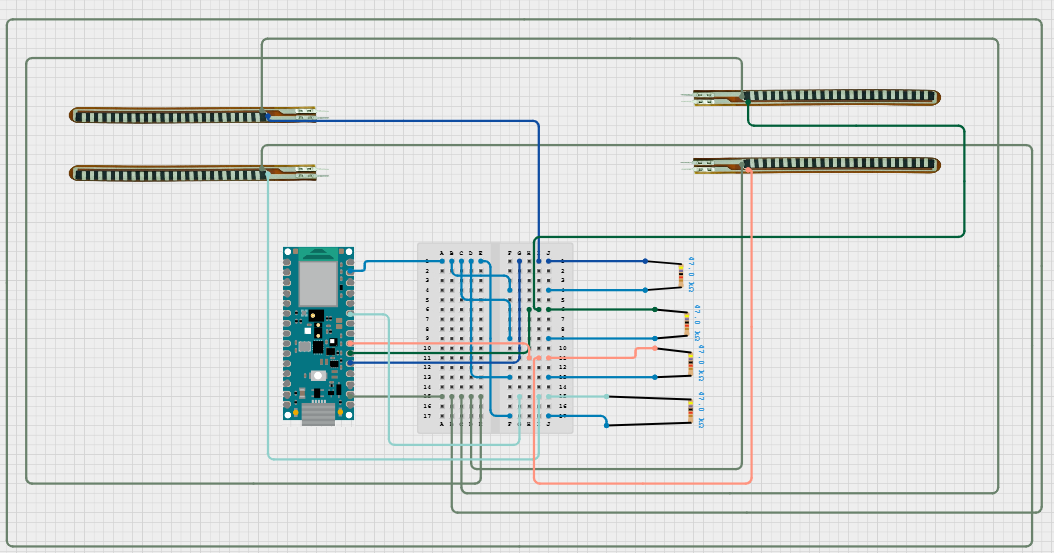
\includegraphics[width=0.9\textwidth]{FYP_Template_Spring/Figures/flex circuit pinout.png}
    \caption{Cuirkit schematic of the flex-sensor interface circuit used for swelling detection.}
    \label{fig:flex_schematic}
\end{figure}

\noindent TO BE CHANGED!! FIGURES ARE TO BE CHANGED BASED ON OUR LAST CONFIG + THE EXPLANATION SHOULD BE MORE DETAILED IF U WANT GUYS BS LA NE3TEMED AAL FINAL DESIGN OF EACH CIRCUIT

\noindent Cuirkit was also used in creating the charging circuit diagram for this system shown in Fig.~\ref{fig:charging_schematic}. This circuit describes how the rechargeable Li-Po battery, the TP4056 charging unit, the microcontroller, and the power conversion unit were connected in the prototype. The diagram proved useful in confirming proper power flow and ensuring that the wearable is powered efficiently and effectively when in use.

\begin{figure}[H]
    \centering
    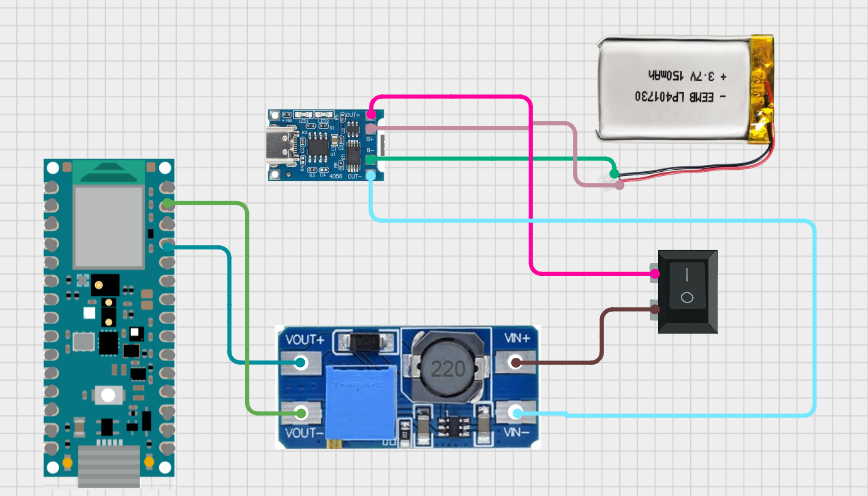
\includegraphics[width=0.55\textwidth]{FYP_Template_Spring/Figures/charging circuit.png}
    \caption{Cuirkit schematic of the charging and power-management circuit of the SoleMate prototype.}
    \label{fig:charging_schematic}
\end{figure} 

\end{comment}

\section{Design Tools}

This section presents the design tools used throughout the development of SoleMate, along with the actual outputs produced by each tool. These include circuit schematics, UI wireframes, and mechanical models that collectively document the design process from early prototyping to final implementation.

\subsection{Circuit Schematic Design --- Cuirkit}

\noindent Cuirkit was used to prepare the circuit schematics and connection diagrams of the main hardware subsystems developed for SoleMate. It provided a clear visual representation of the electrical layout of the prototype, which helped the team organize sensor connections, verify pin assignments, and document the integration of the different modules used throughout the system. The generated schematics were particularly useful during debugging and testing, since they offered a structured reference for wiring, power routing, and subsystem interfacing.

\noindent One of the main schematics created using Cuirkit was the Velostat-based plantar-pressure sensing circuit shown in Fig.~\ref{fig:velostat_schematic}. This schematic illustrates the pressure acquisition setup used to reconstruct plantar-pressure frames from the sensing matrix. The design includes the Velostat sensing layer, the associated conductive traces, and the multiplexing arrangement used to scan the matrix while reducing the number of required microcontroller pins. By organizing the matrix rows and columns through multiplexers, the circuit enables sequential sampling of the pressure nodes and supports the generation of plantar-pressure heatmaps for gait analysis.

\begin{figure}[H]
    \centering
    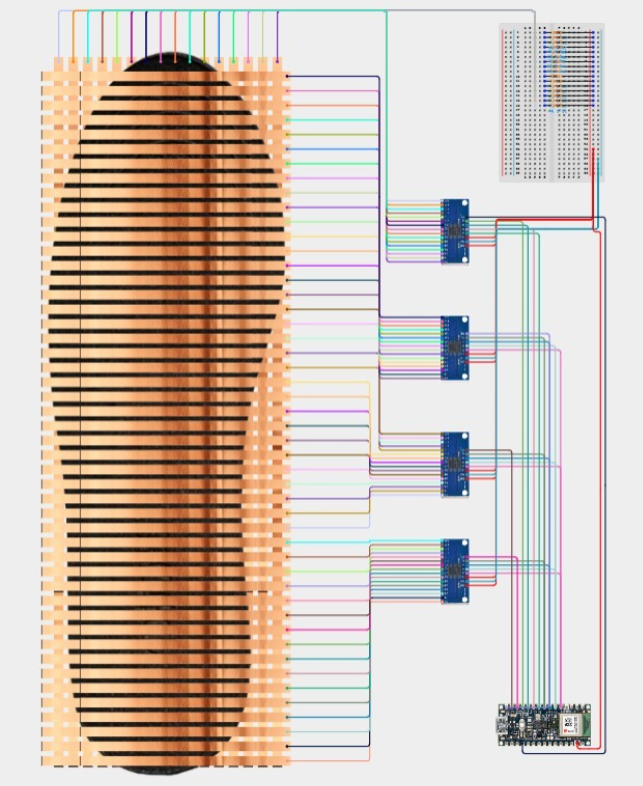
\includegraphics[width=0.82\textwidth]{FYP_Template_Spring/Figures/velostat circuit.png}
    \caption{Cuirkit schematic of the Velostat-based plantar-pressure sensing circuit used for pressure acquisition and heatmap generation.}
    \label{fig:velostat_schematic}
\end{figure}

\noindent Another schematic prepared using Cuirkit was the flex-sensor interface circuit shown in Fig.~\ref{fig:flex_schematic}. This diagram documents the connection of the flex sensors used for swelling detection. The circuit was designed so that changes in flex-sensor resistance could be translated into voltage variations readable by the microcontroller through analog input pins. This schematic helped clarify the resistor connections, signal paths, and sensor interfacing required for the swelling-detection subsystem, making the implementation and testing process more organized.

\begin{figure}[H]
    \centering
    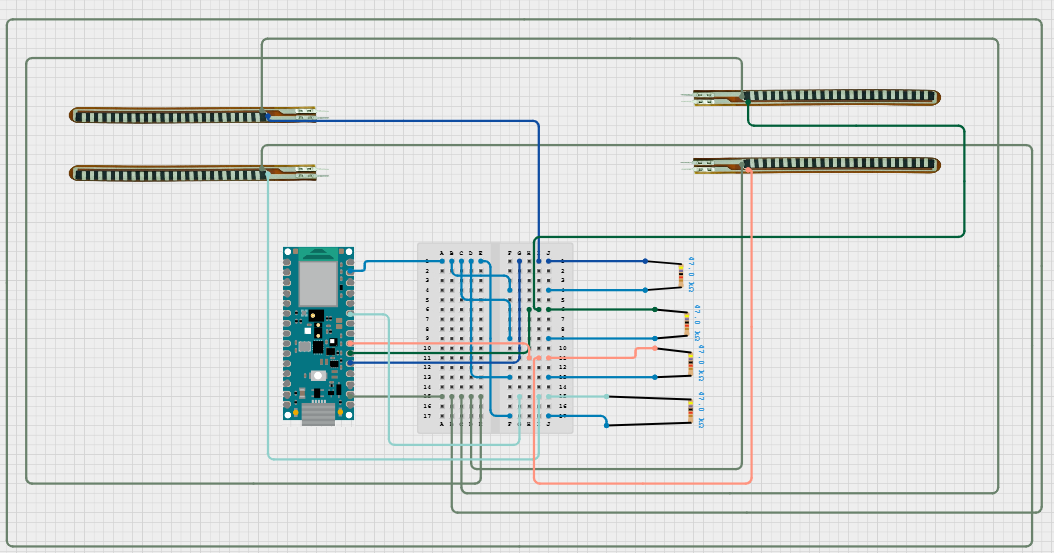
\includegraphics[width=0.9\textwidth]{FYP_Template_Spring/Figures/flex circuit pinout.png}
    \caption{Cuirkit schematic of the flex-sensor interface circuit used for swelling detection.}
    \label{fig:flex_schematic}
\end{figure}


\noindent Cuirkit was also used in creating the charging circuit diagram for this system shown in Fig.~\ref{fig:charging_schematic}. This circuit describes how the rechargeable Li-Po battery, the TP4056 charging unit, the microcontroller, and the power conversion unit were connected in the prototype. The diagram proved useful in confirming proper power flow and ensuring that the wearable is powered efficiently and effectively when in use.

\begin{figure}[H]
    \centering
    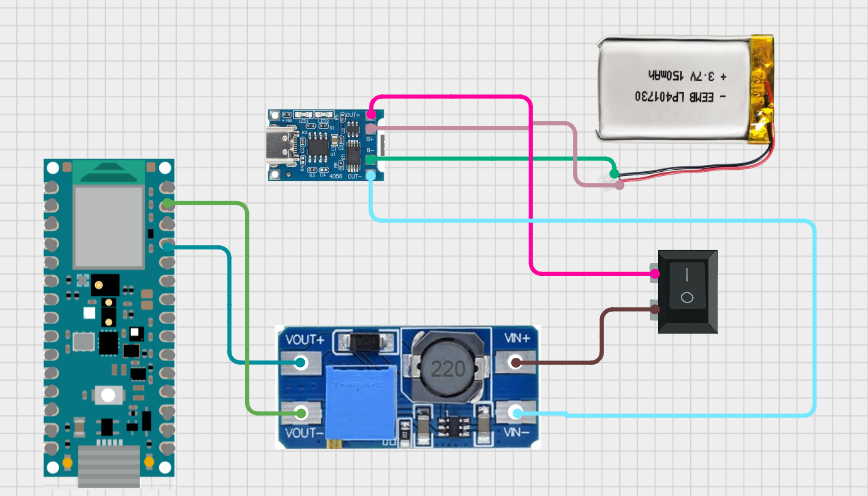
\includegraphics[width=0.55\textwidth]{FYP_Template_Spring/Figures/charging circuit.png}
    \caption{Cuirkit schematic of the charging and power-management circuit of the SoleMate prototype.}
    \label{fig:charging_schematic}
\end{figure}

\subsection{UI/UX Prototyping }

\noindent Visily was used during the early phase of the mobile application design to build the main user interface (UI) and dashboard structure. It supported quick prototyping, which helped establish the initial screen flow and overall visual layout of the app before any implementation in Android Studio. The design prioritized simplicity and ease of use, placing key features such as real-time monitoring, data display, and system status alerts in accessible locations within the interface.

\noindent Fig.~\ref{fig:visily_wireframe} shows the initial wireframe screens produced in Visily. These mockups served as the direct blueprint for the Android Studio implementation, and were revised iteratively based on testing feedback, resulting in updates to the navigation flow, button structure, and screen interactions.

\begin{figure}[H]
    \centering
    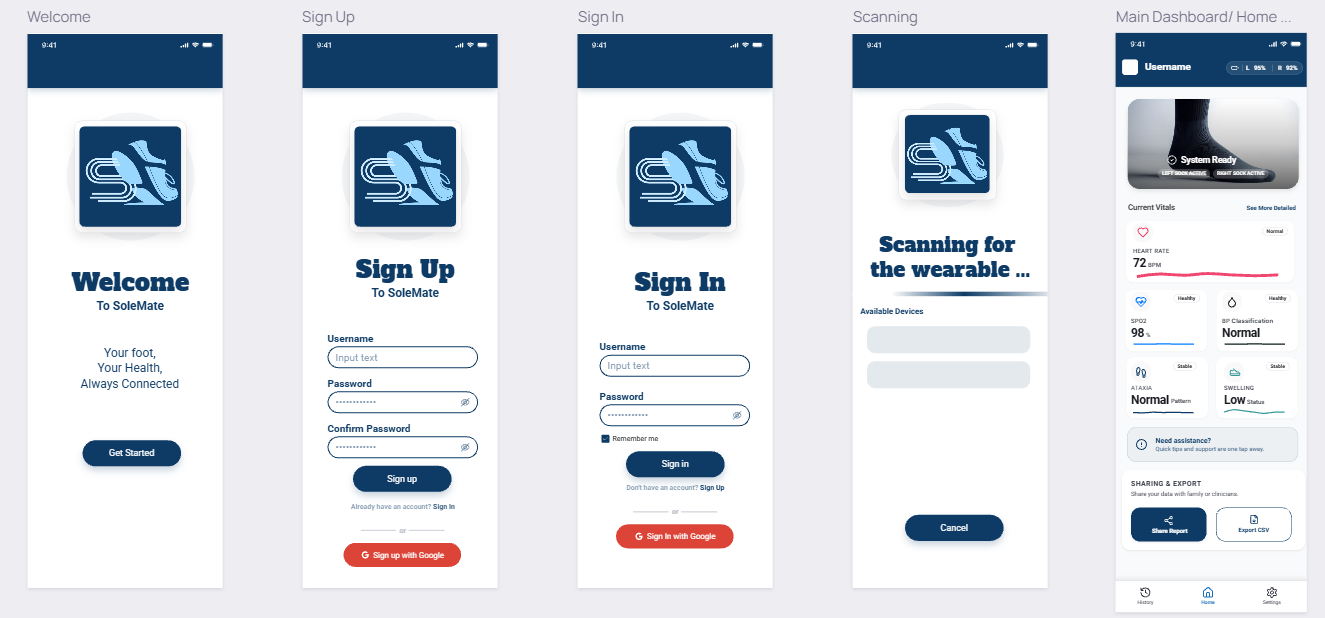
\includegraphics[width=1\textwidth]{FYP_Template_Spring/Figures/visily_wireframe.png}    \caption{Visily wireframe designs showing the initial UI layout and screen flow of the SoleMate mobile application.}
    \label{fig:visily_wireframe}
\end{figure}

\subsection{3D Mechanical Design}

\noindent Fusion 360 was used to design the anatomical foot model that served as. The model was dimensioned to approximate the geometry of an adult foot, providing a consistent and repeatable surface for positioning the Velostat sensing matrix and validating pressure distribution uniformity across sessions. Designing the model in Fusion 360 prior to fabrication allowed the team to verify sensor placement geometry and mounting constraints before committing to the 3D printing process.

\noindent Fig.~\ref{fig:fusion_foot} shows the Fusion 360 CAD model of the foot prototype.

\begin{figure}[H]
    \centering
    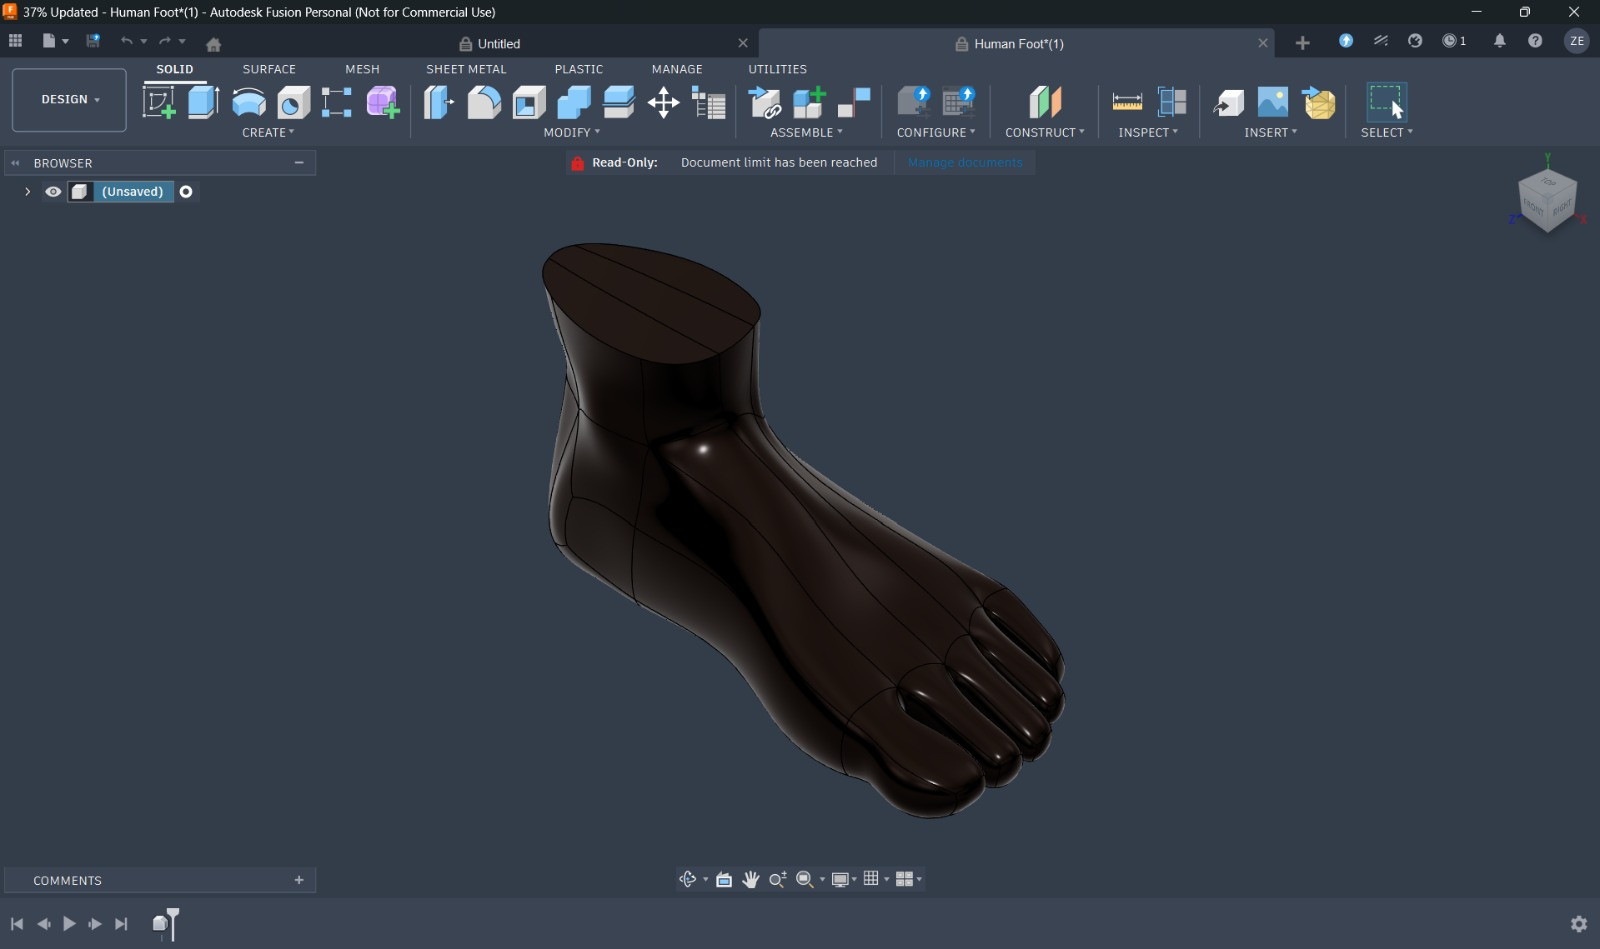
\includegraphics[width=1\textwidth]{FYP_Template_Spring/Figures/fusion_foot.png}
    \caption{Fusion 360 CAD model of the anatomical foot prototype designed for sensor calibration and plantar pressure testing.}
    \label{fig:fusion_foot}
\end{figure}

\subsection{3D-Printed Foot Prototype}

\noindent The foot model designed in Fusion 360 was fabricated using a 3D printer available in the university laboratory. The printed prototype provided a stable, human-independent platform for repeatable sensor calibration, eliminating variability introduced by testing directly on human subjects during early development stages. It was used specifically to validate the spatial layout of the Velostat pressure matrix, assess contact uniformity, and generate reference plantar pressure frames for AI model development.

\noindent Fig.~\ref{fig:printed_foot} shows the fabricated 3D-printed foot prototype used during the calibration and testing phases.

\begin{figure}[H]
    \centering
    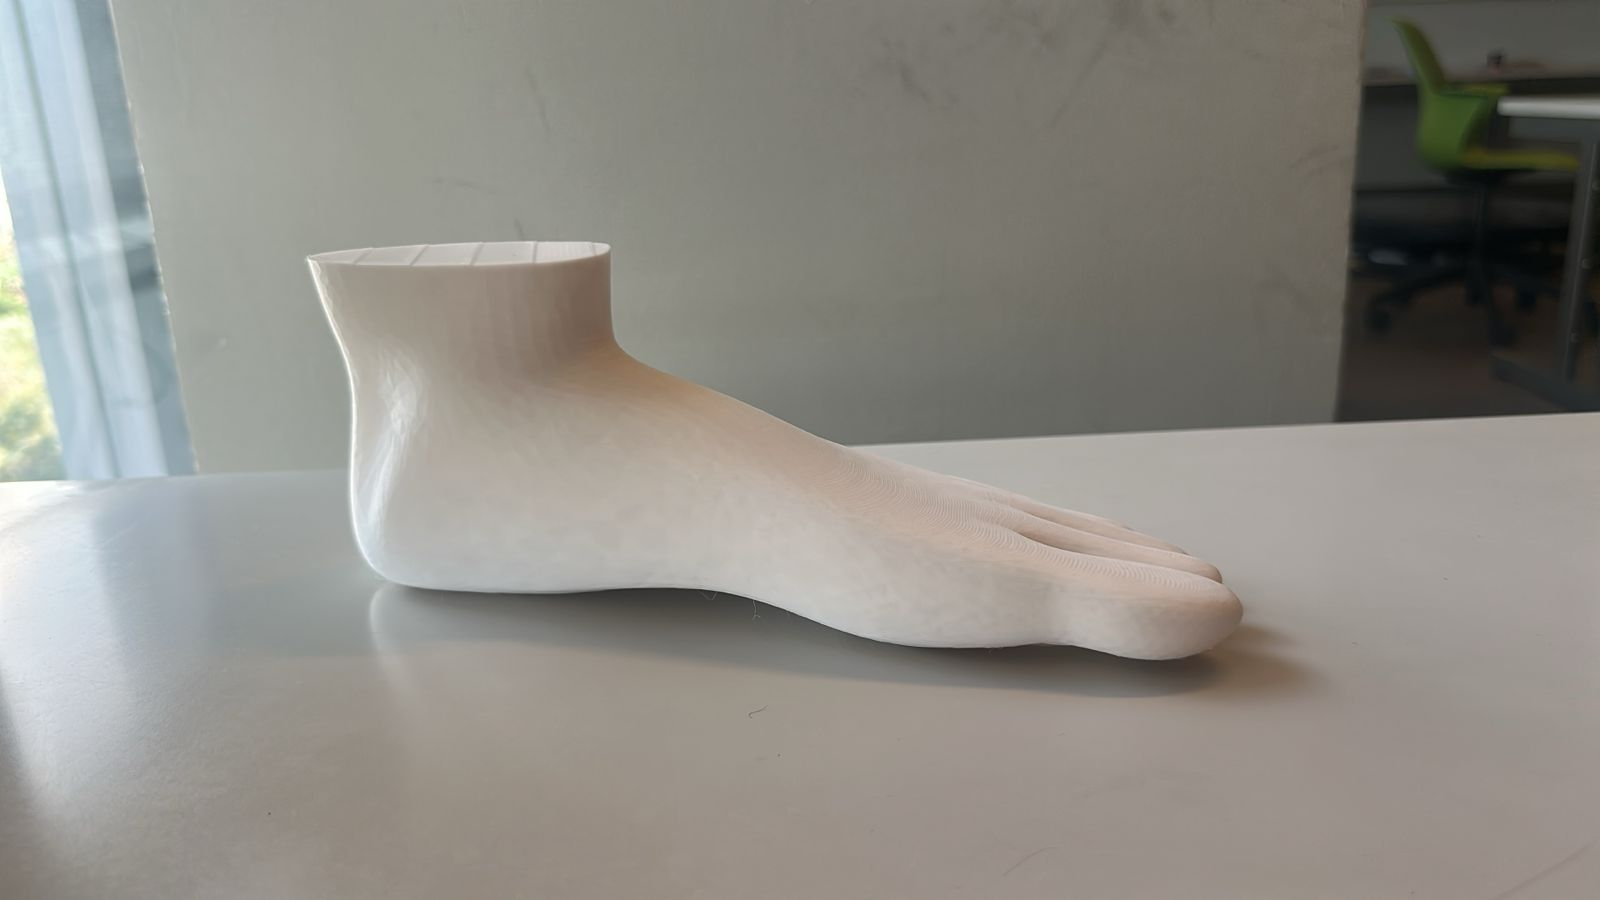
\includegraphics[width=1\textwidth]{FYP_Template_Spring/Figures/printed_foot.png}
    % TO BE ADDED: replace with your photo of the actual printed foot
    \caption{3D-printed anatomical foot prototype used for plantar pressure sensor calibration and system testing.}
    \label{fig:printed_foot}
\end{figure}

\section{Remarks}

All listed resources contribute to the successful development and testing of the SoleMate wearable system. The team began with sensor calibration and BLE communication before progressing toward machine learning integration and dashboard development. New tools such as Google Colab, Android Studio, and SendGrid were adopted iteratively as the project scope expanded to include cloud connectivity and mobile application delivery. GitHub Copilot proved particularly valuable input during Android development, where the team had limited prior experience with the framework. Tools such as MATLAB and Python introduced new learning opportunities for advanced biomedical signal processing and AI-based diagnostic modeling.
